\documentclass[tikz,border=5]{standalone}
\usepackage[utf8x]{inputenc}
\usepackage[T1]{fontenc}
\usepackage{amsmath}
\usepackage{amssymb}
\usepackage{color}
\usepackage[]{xcolor}
\usepackage{tikz}
\usepackage{tikz}
\usepackage{tikz-feynman}
\tikzfeynmanset{warn luatex=false}

\begin{document}

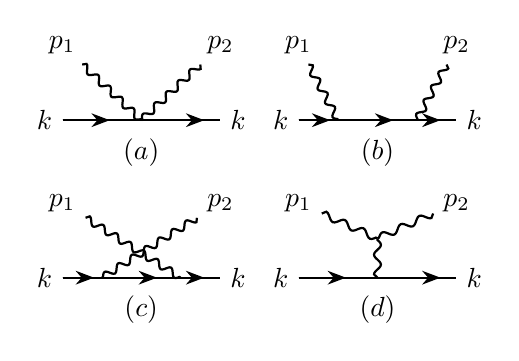
\begin{tikzpicture}[thick, transform shape]
\begin{feynman}
%%Second
\vertex(ce);
\vertex [below = 0.1 of ce] (ce01){\((b)\)};
\vertex [left = 0.5 of ce] (l01);
\vertex [right = 0.5 of ce] (r01);
\vertex [above = 1 of ce] (c02);
\vertex [left = 1 of ce] (c12){\(k\)};
\vertex [right = 1 of ce] (c22){\(k\)};
\vertex [above left = 1 of ce] (c32){\(p_1\)};
\vertex [above right = 1 of ce] (c42){\(p_2\)};

\vertex[left = 3 of ce](ce2);
\vertex [below = 0.1 of ce2] (ce02){\((a)\)};
\vertex [above = 1 of ce2] (c01);
\vertex [left = 1 of ce2] (c11){\(k\)};
\vertex [right = 1 of ce2] (c21){\(k\)};
\vertex [above left = 1 of ce2] (c31){\(p_1\)};
\vertex [above right = 1 of ce2] (c41){\(p_2\)};

%%Third
\vertex[below = 2 of ce2](ce3);
\vertex [below = 0.1 of ce3] (ce03){\((c)\)};
\vertex [left = 0.5 of ce3] (l02);
\vertex [right = 0.5 of ce3] (r02);

\vertex [above = 1 of ce3] (c03);
\vertex [left = 1 of ce3] (c13){\(k\)};
\vertex [right = 1 of ce3] (c23){\(k\)};
\vertex [above left = 1 of ce3] (c33){\(p_1\)};
\vertex [above right = 1 of ce3] (c43){\(p_2\)};

%%FOurth
\vertex[below = 2 of ce](ce4);
\vertex [below = 0.1 of ce4] (ce04){\((d)\)};
\vertex[above = 0.5 of ce4](ce5);

\vertex [above = 1 of ce4] (c04);
\vertex [left = 1 of ce4] (c14){\(k\)};
\vertex [right = 1 of ce4] (c24){\(k\)};
\vertex [above left = 1 of ce4] (c34){\(p_1\)};
\vertex [above right = 1 of ce4] (c44){\(p_2\)};

\diagram* {
(c12)--(c22),
(c11) --(c21),
(c13) --(c23),
(c14) --(c24),
(ce2) - - [boson, edge label'=\(\)](c31),
(ce2) - - [boson, edge label'=\(\)](c41),
(l01)- - [boson, edge label'=\(\)](c32),
(r01)- - [boson, edge label'=\(\)](c42),
(l02)- - [boson, edge label'=\(\)](c43),
(r02)- - [boson, edge label'=\(\)](c33),
(ce5)- - [boson, edge label'=\(\)](ce4),
(ce5)- - [boson, edge label'=\(\)](c34),
(ce5)- - [boson, edge label'=\(\)](c44),
};
\begin{scope}[decoration={
		markings,
		mark=at position 0.6 with {\arrow[>=Stealth]{>}}}] 
\draw[postaction={decorate}] (c12) -- node [right=4pt] {}(c22);
\draw[postaction={decorate}] (c13) -- node [right=4pt] {}(c23);
\end{scope}
\begin{scope}[decoration={
		markings,
		mark=at position 0.3 with {\arrow[>=Stealth]{>}}}] 
\draw[postaction={decorate}] (c11) -- node [right=4pt] {}(c21);
\draw[postaction={decorate}] (c14) -- node [right=4pt] {}(c24);
\end{scope}
\begin{scope}[decoration={
		markings,
		mark=at position 0.9 with {\arrow[>=Stealth]{>}}}] 
\draw[postaction={decorate}] (c11) -- node [right=4pt] {}(c21);
\draw[postaction={decorate}] (c14) -- node [right=4pt] {}(c24);
\end{scope}
\begin{scope}[decoration={
		markings,
		mark=at position 0.2 with {\arrow[>=Stealth]{>}}}] 
\draw[postaction={decorate}] (c12) -- node [right=4pt] {}(c22);
\draw[postaction={decorate}] (c13) -- node [right=4pt] {}(c23);
\end{scope}
\begin{scope}[decoration={
		markings,
		mark=at position 0.9 with {\arrow[>=Stealth]{>}}}] 
\draw[postaction={decorate}] (c12) -- node [right=4pt] {}(c22);
\draw[postaction={decorate}] (c13) -- node [right=4pt] {}(c23);
\end{scope}
\end{feynman}
\end{tikzpicture}

\end{document}